\documentclass{article}

\usepackage{tikz}
\usepackage{float}
\usepackage{multirow}
\usepackage{rotating}
\usepackage[margin=1in]{geometry}


\graphicspath{ {./images} }
\pagenumbering{gobble}

\title{
    Manutenção Inteligente em Cenário de Indústria 4.0 \\
    \vspace{0.75em}
    \Large Entrega 4 \\  \vspace{1.25em} 
    \large
    \begin{tabular}{rl}
        \textbf{Turno:}& MODL03 \\ 
        \rule{0pt}{1.25em} 
        \textbf{Docente:}& Maria do Rosário Bernardo 
    \end{tabular}
}
\author{}
\date{}


\begin{document}
    \maketitle
    \begin{tikzpicture}[overlay, remember picture]
        \node[xshift=3.5cm,yshift=-2.5cm] at (current page.north west) {
\includegraphics[scale = 0.35]{logo_ist.jpeg}};
    \end{tikzpicture}
    \vspace{-1.2cm}
    \begin{table}[H]
        \centering
        \begin{tabular}{|l|l|l|l|l}
        \cline{1-4}
        \multicolumn{1}{|l|}{}                   & \multicolumn{1}{l|}{}       & \multicolumn{1}{l|}{}                             & \multicolumn{1}{l|}{}                   &  \\
        \multicolumn{1}{|l|}{}                   & \multicolumn{1}{l|}{}       & \multicolumn{1}{l|}{}                             & \multicolumn{1}{l|}{}                   &  \\
        \multicolumn{1}{|c|}{Nome}               & \multicolumn{1}{c|}{Número} & \multicolumn{1}{c|}{Esforço estimado de trabalho} & \multicolumn{1}{c|}{Tarefas realizadas} &  \\
        \multicolumn{1}{|l|}{}                   & \multicolumn{1}{l|}{}       & \multicolumn{1}{l|}{}                             & \multicolumn{1}{l|}{}                   &  \\
        \multicolumn{1}{|l|}{}                   & \multicolumn{1}{l|}{}       & \multicolumn{1}{l|}{}                             & \multicolumn{1}{l|}{}                   &  \\ \cline{1-4}
        \multicolumn{1}{|l|}{}                   & \multicolumn{1}{l|}{}       & \multicolumn{1}{l|}{}                             & \multirow{5}{7cm}{Correção dos diagramas da entrega 3. Realização do bdd, ibd e diagrama de máquina de estados, tendo assegurado a coerência entre os diversos diagramas.}                   &  \\
        \multicolumn{1}{|l|}{}                   & \multicolumn{1}{l|}{}       & \multicolumn{1}{l|}{}                             & \multicolumn{1}{l|}{}                   &  \\
        \multicolumn{1}{|c|}{António Coelho}     & \multicolumn{1}{c|}{95535}  & \multicolumn{1}{c|}{28 horas}                     & \multicolumn{1}{l|}{}                   &  \\
        \multicolumn{1}{|l|}{}                   & \multicolumn{1}{l|}{}       & \multicolumn{1}{l|}{}                             & \multicolumn{1}{l|}{}                   &  \\
        \multicolumn{1}{|l|}{}                   & \multicolumn{1}{l|}{}       & \multicolumn{1}{l|}{}                             & \multicolumn{1}{l|}{}                   & \\ \cline{1-4}
        \multicolumn{1}{|l|}{}                   & \multicolumn{1}{l|}{}       & \multicolumn{1}{l|}{}                             & \multirow{5}{7cm}{Correção dos diagramas das entregas 1 e 2. Realização dos diagramas de sequência e de máquina de estados, tendo assegurado a coerência entre diagramas.}                   &   \\
        \multicolumn{1}{|l|}{}                   & \multicolumn{1}{l|}{}       & \multicolumn{1}{l|}{}                             & \multicolumn{1}{l|}{}                   &  \\
        \multicolumn{1}{|c|}{Sebastião Assunção} & \multicolumn{1}{c|}{95536}  & \multicolumn{1}{c|}{28 horas}                     & \multicolumn{1}{l|}{}                   &  \\
        \multicolumn{1}{|l|}{}                   & \multicolumn{1}{l|}{}       & \multicolumn{1}{l|}{}                             & \multicolumn{1}{l|}{}                   &  \\
        \multicolumn{1}{|l|}{}                   & \multicolumn{1}{l|}{}       & \multicolumn{1}{l|}{}                             & \multicolumn{1}{l|}{}                   &  \\ \cline{1-4}
        \multicolumn{1}{|l|}{}                   & \multicolumn{1}{l|}{}       & \multicolumn{1}{l|}{}                             & \multirow{5}{7cm}{Correção dos diagramas das entregas 1 e 2. Realização dos diagramas de sequência e de máquina de estados, tendo assegurado a coerência entre diagramas.}                   &  \\
        \multicolumn{1}{|l|}{}                   & \multicolumn{1}{l|}{}       & \multicolumn{1}{l|}{}                             & \multicolumn{1}{l|}{}                   &  \\
        \multicolumn{1}{|c|}{Duarte Almeida}     & \multicolumn{1}{c|}{95565}  & \multicolumn{1}{c|}{28 horas}                     & \multicolumn{1}{l|}{}                   &  \\
        \multicolumn{1}{|l|}{}                   & \multicolumn{1}{l|}{}       & \multicolumn{1}{l|}{}                             & \multicolumn{1}{l|}{}                   &  \\
        \multicolumn{1}{|l|}{}                   & \multicolumn{1}{l|}{}       & \multicolumn{1}{l|}{}                             & \multicolumn{1}{l|}{}                   &  \\ \cline{1-4}
        \multicolumn{1}{|l|}{}                   & \multicolumn{1}{l|}{}       & \multicolumn{1}{l|}{}                             & \multirow{5}{7cm}{Correção dos diagramas da entrega 3. Realização do bdd, ibd e diagrama de máquina de estados, tendo assegurado a coerência entre os diversos diagramas.}                   &  \\
        \multicolumn{1}{|l|}{}                   & \multicolumn{1}{l|}{}       & \multicolumn{1}{l|}{}                             & \multicolumn{1}{l|}{}                   &  \\
        \multicolumn{1}{|c|}{Gustavo Aguiar}     & \multicolumn{1}{c|}{95587}  & \multicolumn{1}{c|}{28 horas}                     & \multicolumn{1}{l|}{}                   &  \\
        \multicolumn{1}{|l|}{}                   & \multicolumn{1}{l|}{}       & \multicolumn{1}{l|}{}                             & \multicolumn{1}{l|}{}                   &  \\
        \multicolumn{1}{|l|}{}                   & \multicolumn{1}{l|}{}       & \multicolumn{1}{l|}{}                             & \multicolumn{1}{l|}{}                   & \\ \cline{1-4}
        \end{tabular}
        \end{table}

    \vspace{0.5cm}

    \noindent \large \textbf{Comentários aos diagramas}

    \vspace{0.4cm}
    \normalsize

    A condição (a) nos diagramas BPMN é verdadeira se e só se  a máquina estava a ser usada por arPRO quando o evento de início da primeira execução do processo foi gerado ou a máquina tem uso por arPRO previsto para as 24h seguintes.

    %Ao nível do modelo de domínio, representaram-se as mensagens com dados de estado das máquinas como não estruturadas pelas unidades a que esses dados remetem. No entanto, abre-se posterior possibilidade comportamental de estruturação ao associar estas mensagens à máquina, que é por sua vez composta pelas suas unidades. \\ \indent
    %A associação do evento de início de manutenção "AvariaInferida" a "DadosEstado" e, indiretamente, a "Máquina" abre também possibilidade comportamental de, assumindo o acesso à data atual por parte da uma máquina, inferir uma avaria (por exemplo, analisando as datas das mensagens recebidas, o intervalo de tempo máximo permitido entre mensagens e as manutenções agendadas/em curso).

    \pagebreak
    \pdfpageattr\expandafter{\the\pdfpageattr/Rotate -90}

    \begin{figure}[H]
        \centering
        \vspace*{1.8cm}
        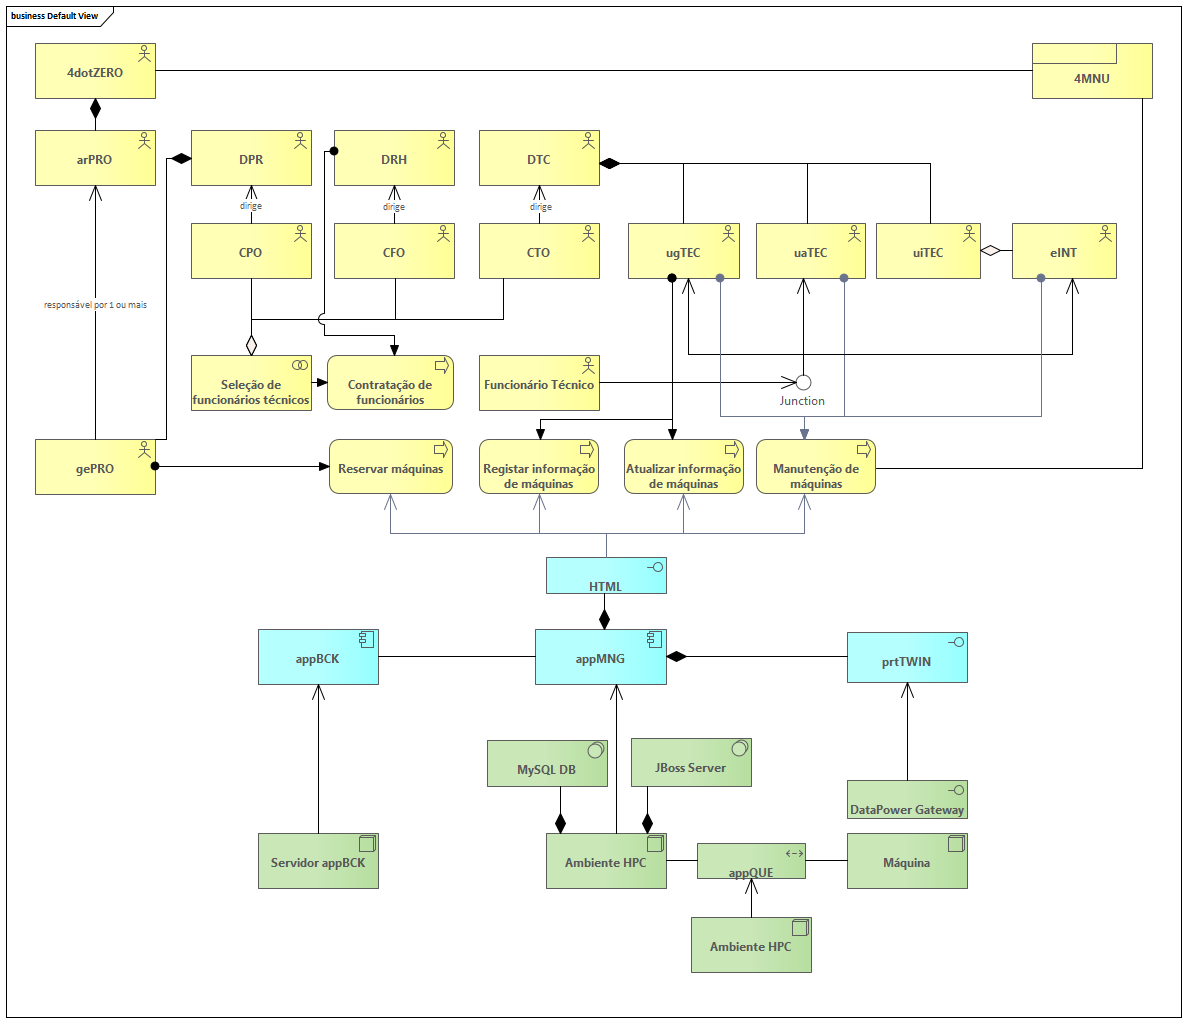
\includegraphics[angle=-90,origin=c,width=\textwidth,height=\textheight,keepaspectratio]{ArchiMate.png}
    \end{figure}

    \pagebreak
    \begin{figure}[H]
        \centering
        \vspace*{-1.4cm}
        \hspace*{-1.2cm}
        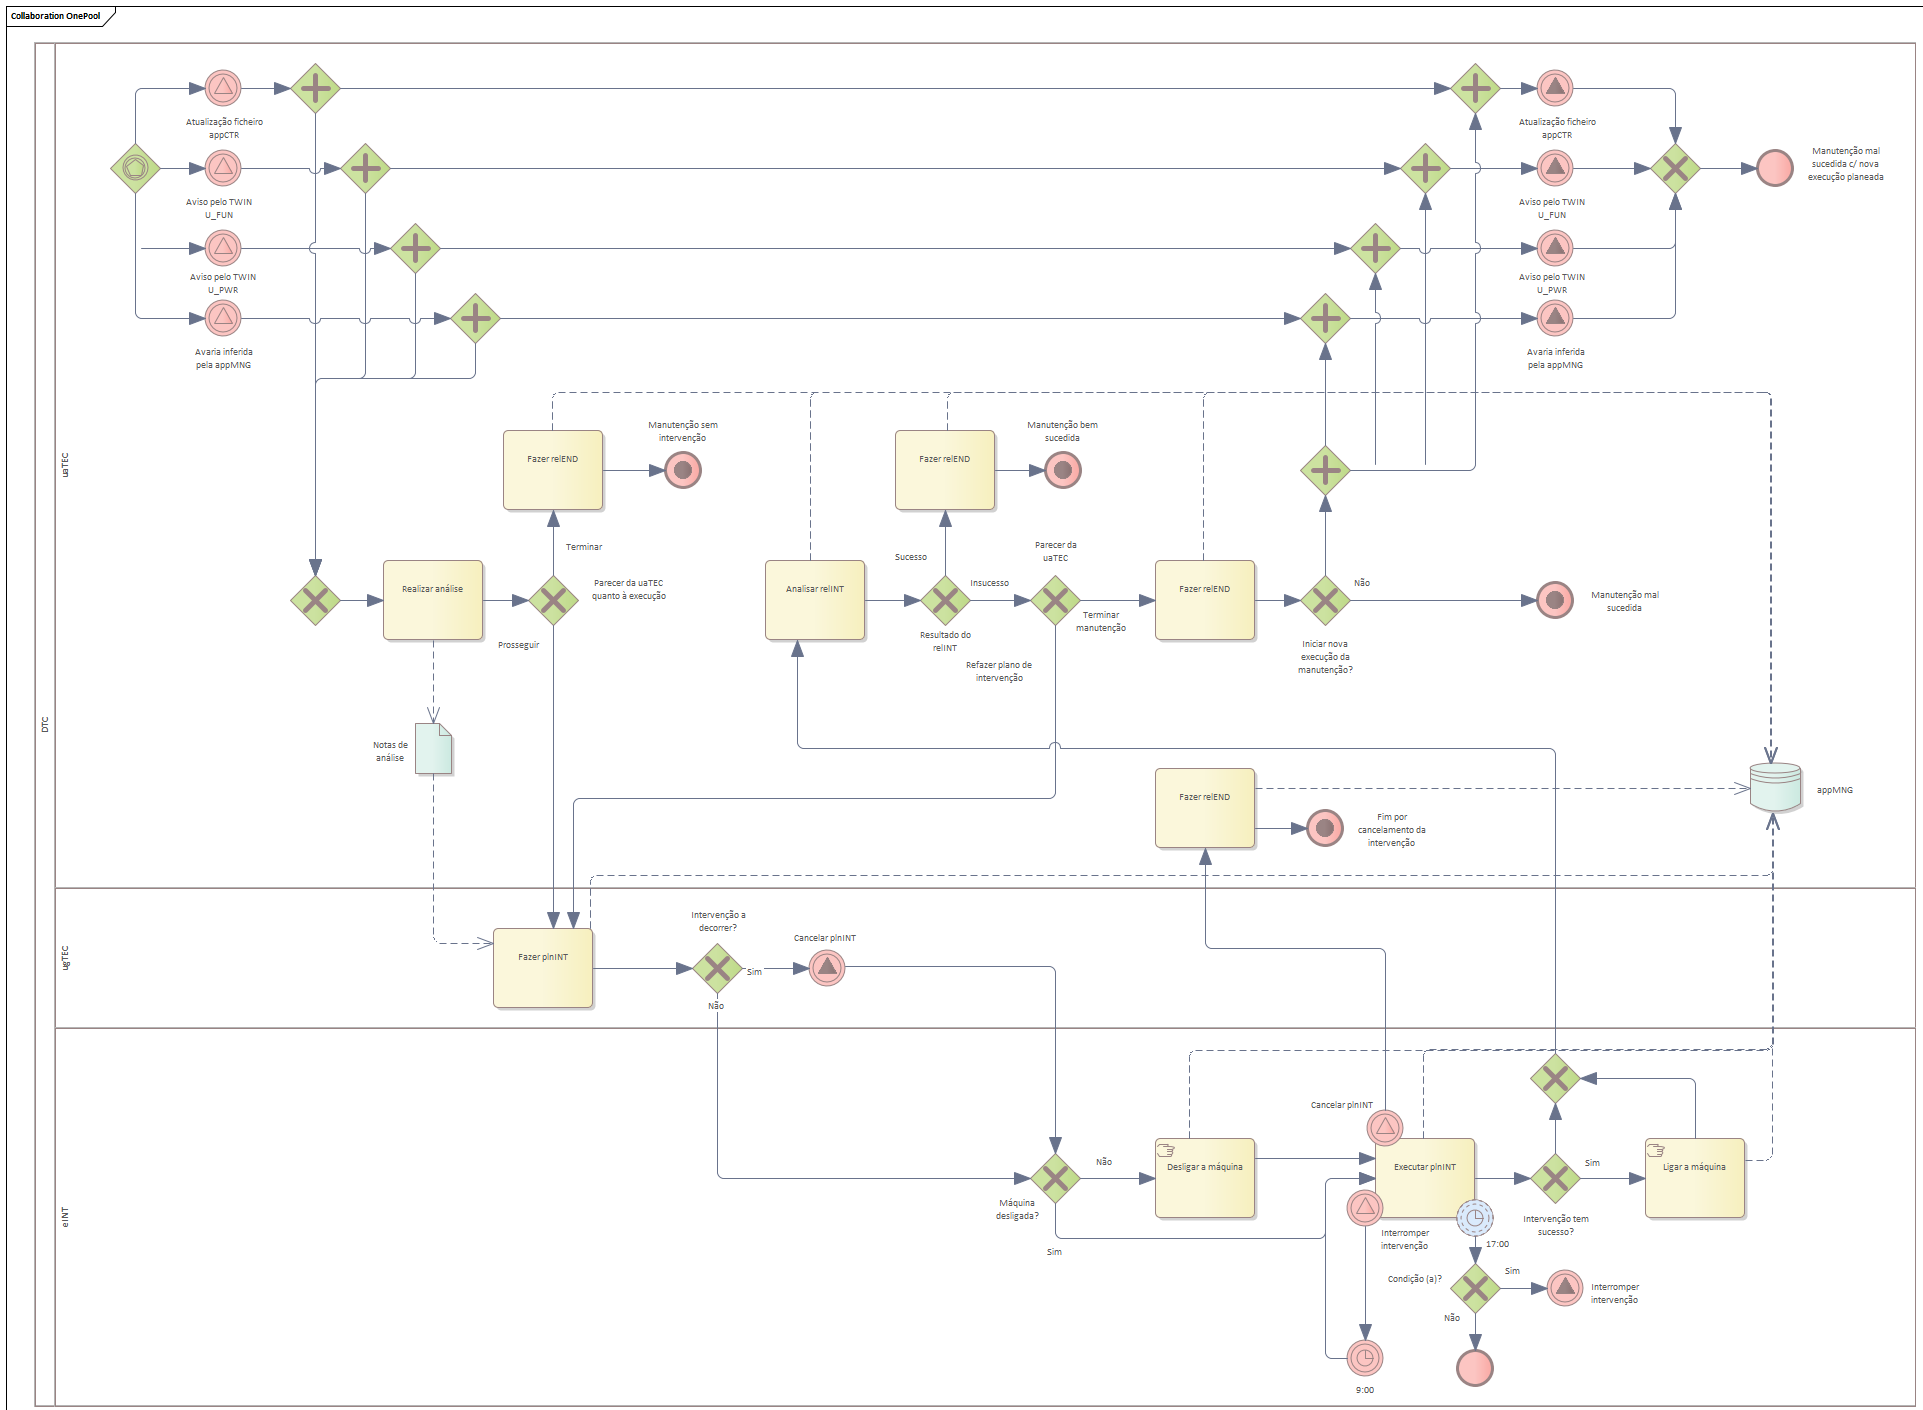
\includegraphics[angle=-90,origin=c, scale=0.50]{BPMN_One_Pool.png}
    \end{figure}
%
    \pagebreak
    \begin{figure}[H]
        \centering
        \vspace*{-1.4cm}
        \hspace*{-1.8cm}
        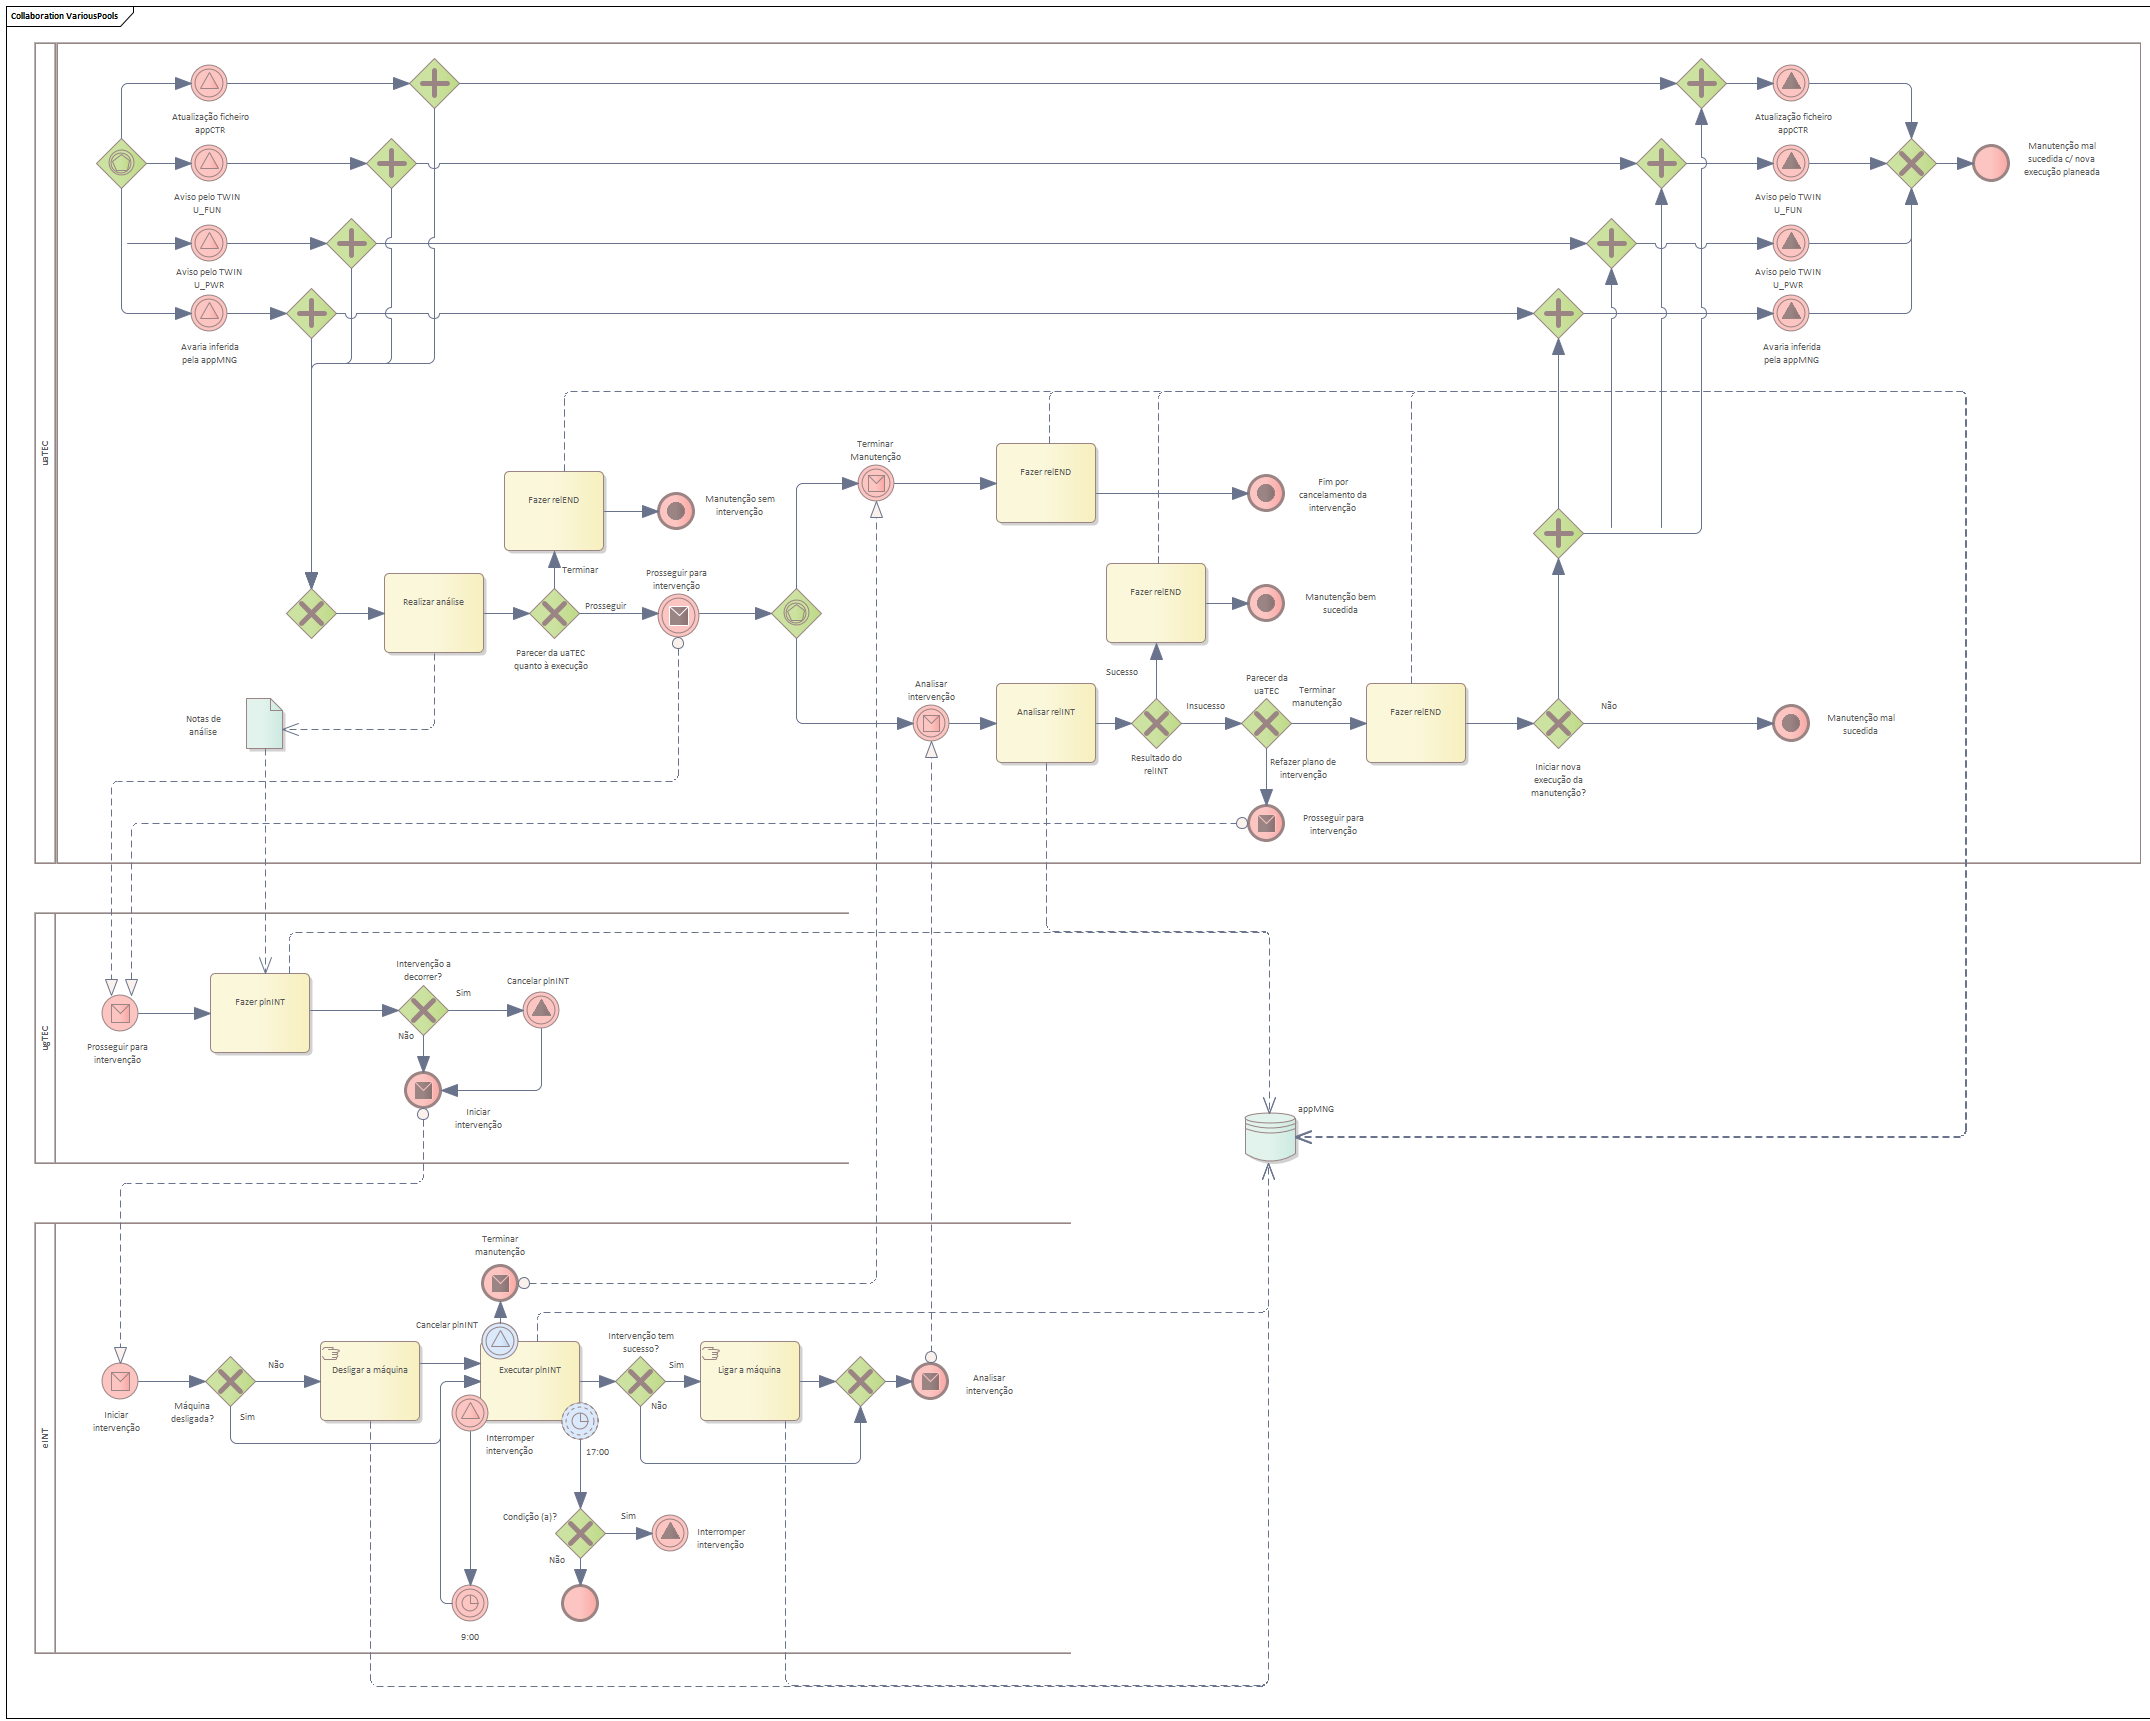
\includegraphics[angle=-90,origin=c, scale=0.45]{BPMN_Various_Pools.png}
    \end{figure}
%
    \pagebreak
    \begin{figure}[H]
        \centering
        \vspace*{1.1cm}
        %\hspace*{-1.75cm}
        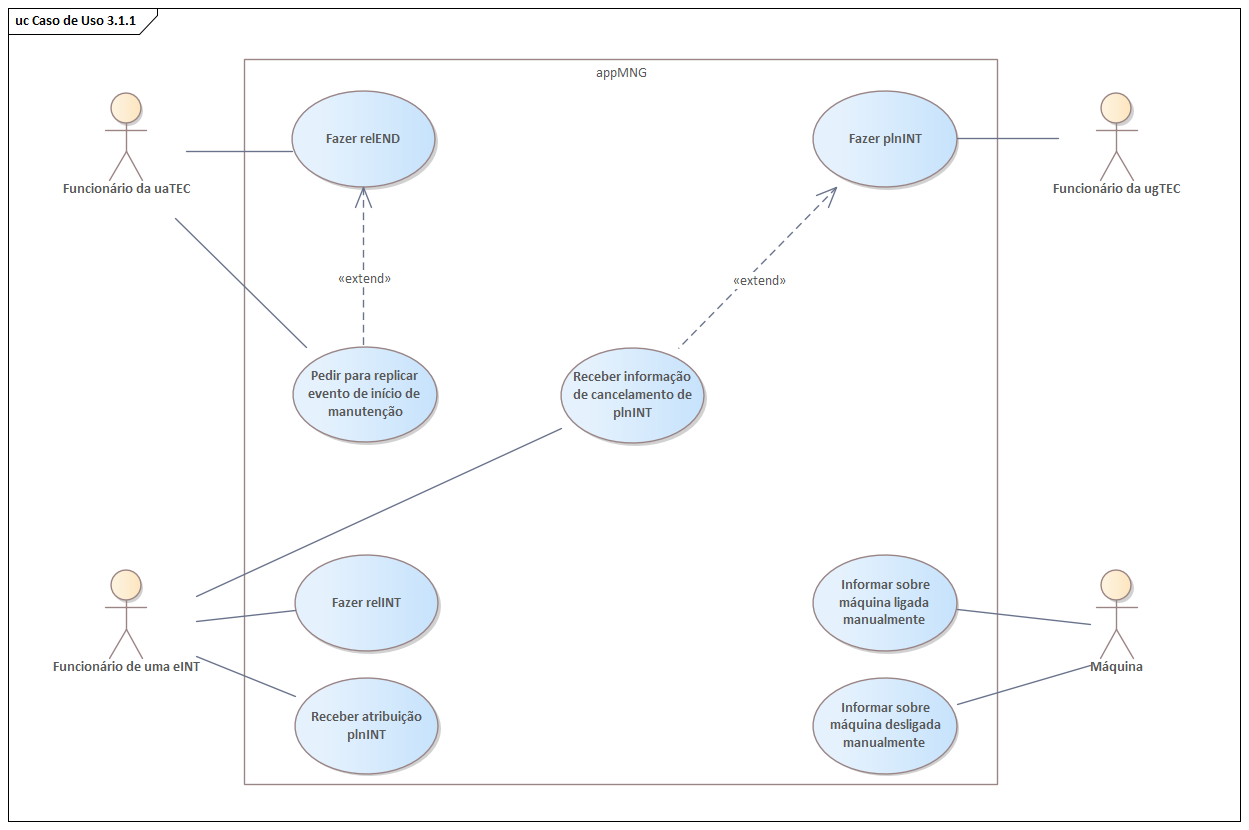
\includegraphics[origin=c, angle=-90, scale=0.85]{1st_Use_Case.png}
    \end{figure}

    \pagebreak
    \begin{figure}[H]
        \centering
        \vspace*{-0.2cm}
        %\hspace*{-1.75cm}
        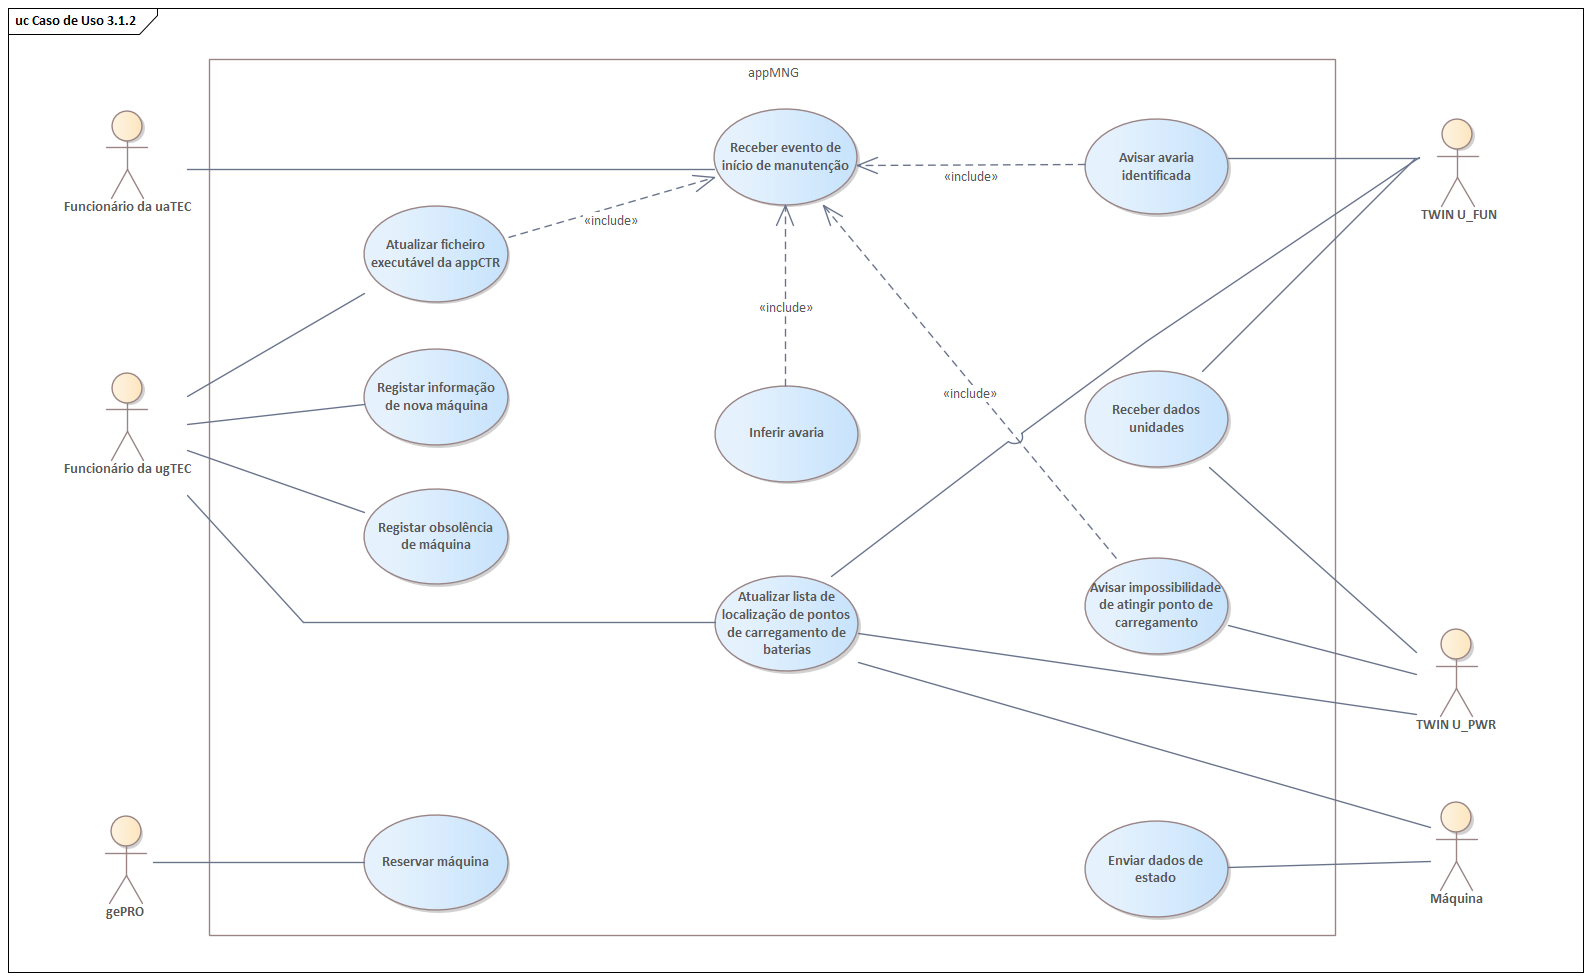
\includegraphics[origin=c, angle=-90, scale=0.75]{2nd_Use_Case.png}
    \end{figure}

    \begin{figure}[H]
        \centering
        \vspace*{1.4cm}
        %\hspace*{-1.75cm}
        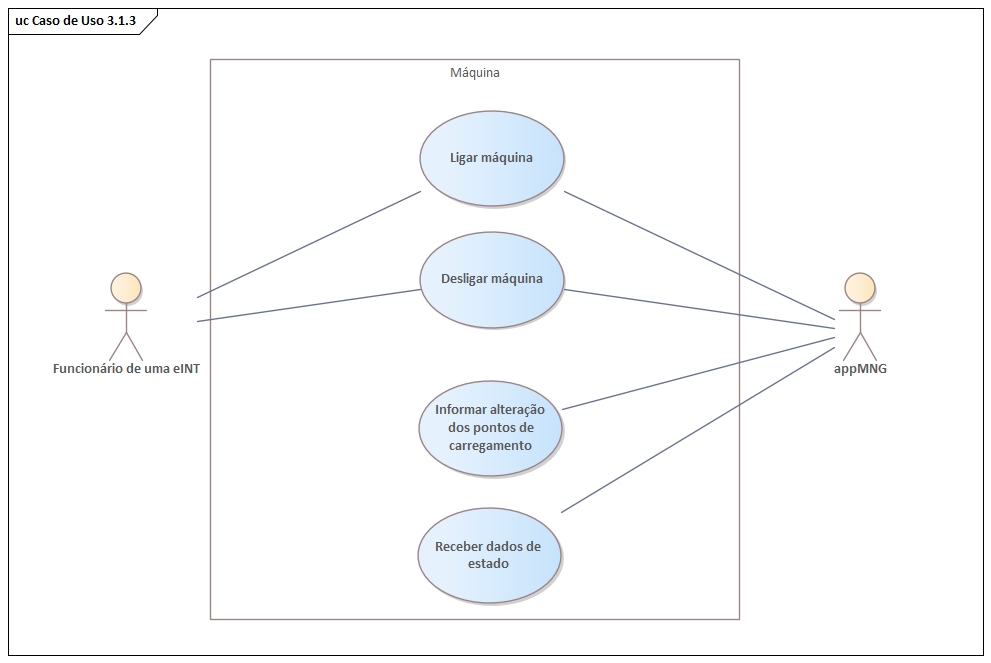
\includegraphics[origin=c, angle=-90]{3rd_Use_Case.png}
    \end{figure}

    \begin{figure}[H]
        \centering
        \vspace*{1.4cm}
        \hspace*{-1.75cm}
        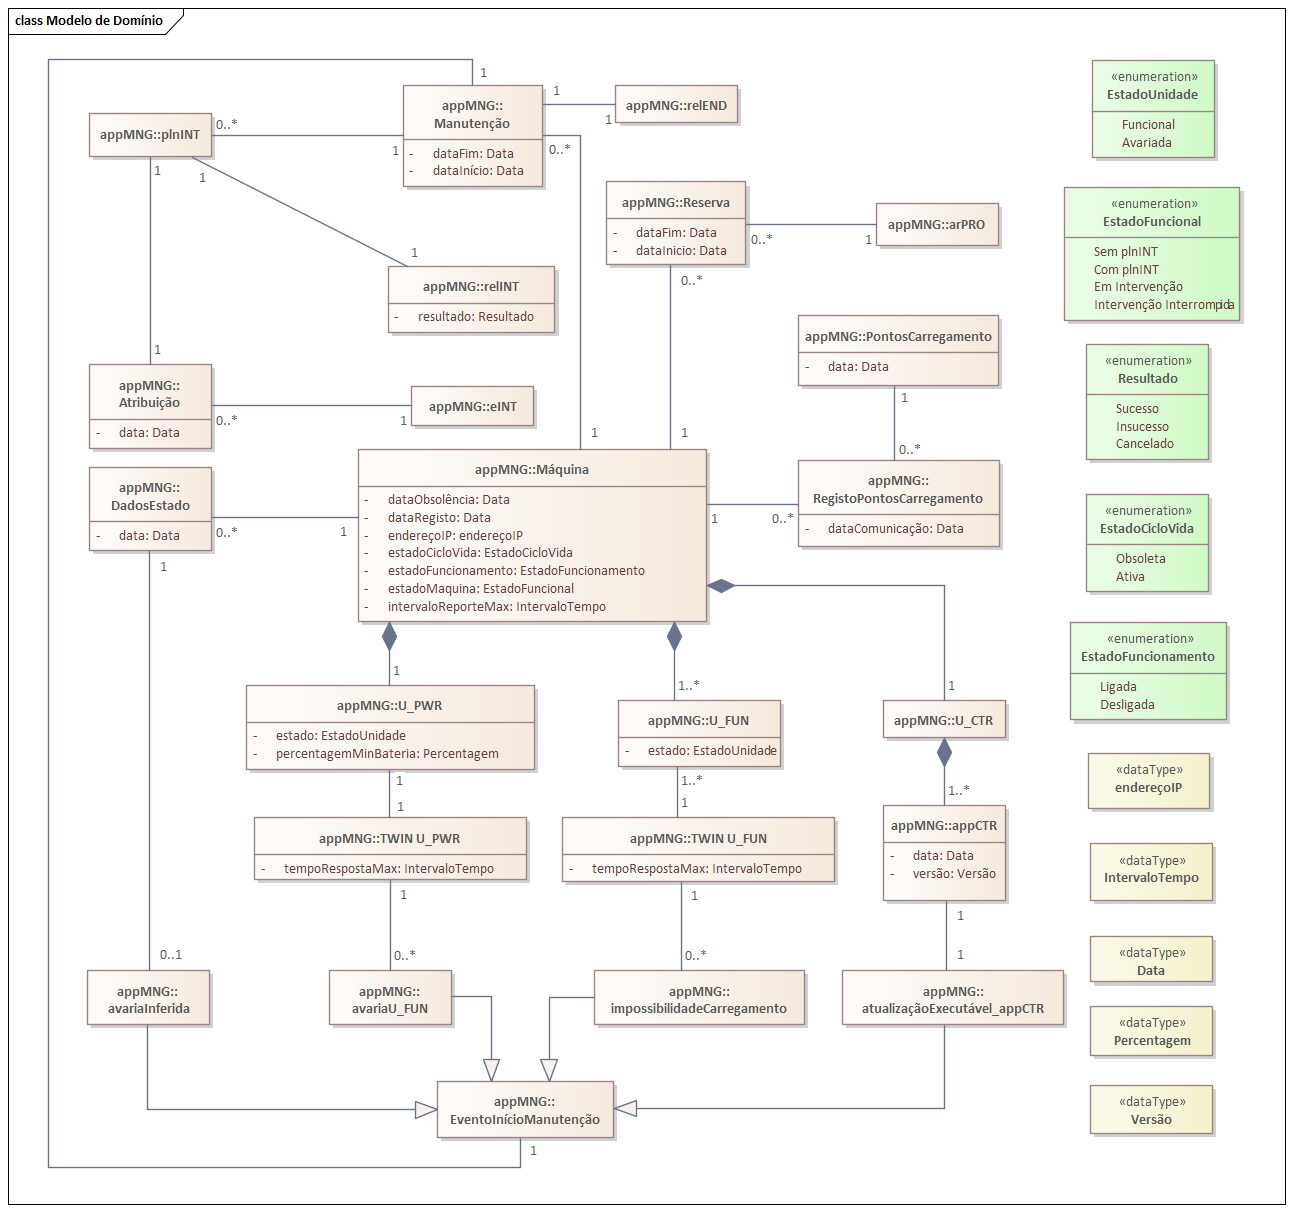
\includegraphics[origin=c, angle=-90, scale = 0.8]{Domain_Model.png}
    \end{figure}

    \begin{figure}[H]
        \centering
        \vspace*{1.4cm}
        %\hspace*{-1.75cm}
        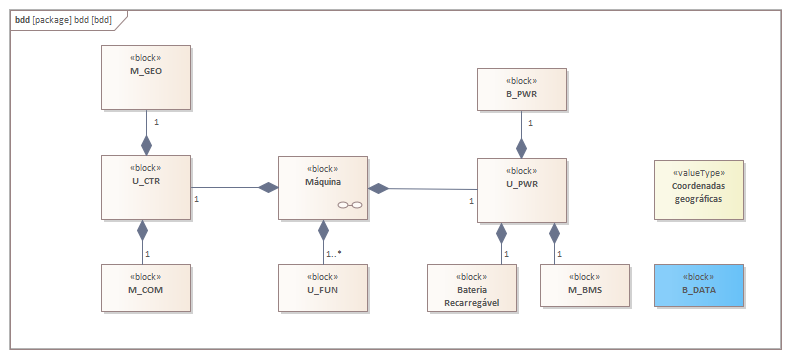
\includegraphics[origin=c, angle=-90]{BDD.png}
    \end{figure}

    \begin{figure}[H]
        \centering
        \vspace*{1.4cm}
        %\hspace*{-1.75cm}
        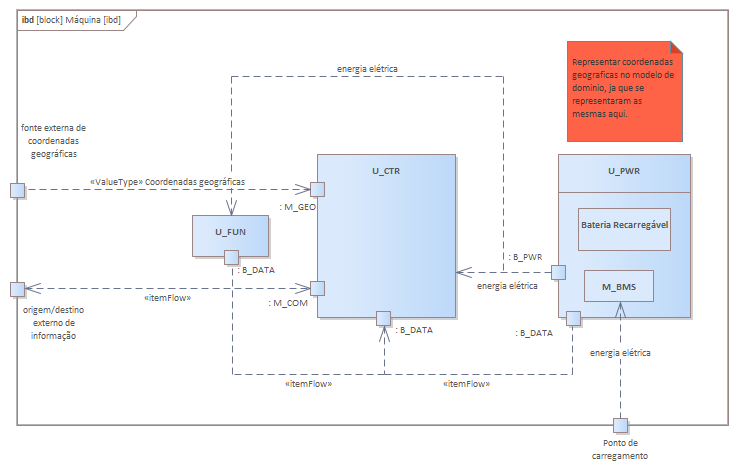
\includegraphics[origin=c, angle=-90]{IBD.png}
    \end{figure}

    \begin{figure}[H]
        \centering
        \vspace*{1.4cm}
        %\hspace*{-1.75cm}
        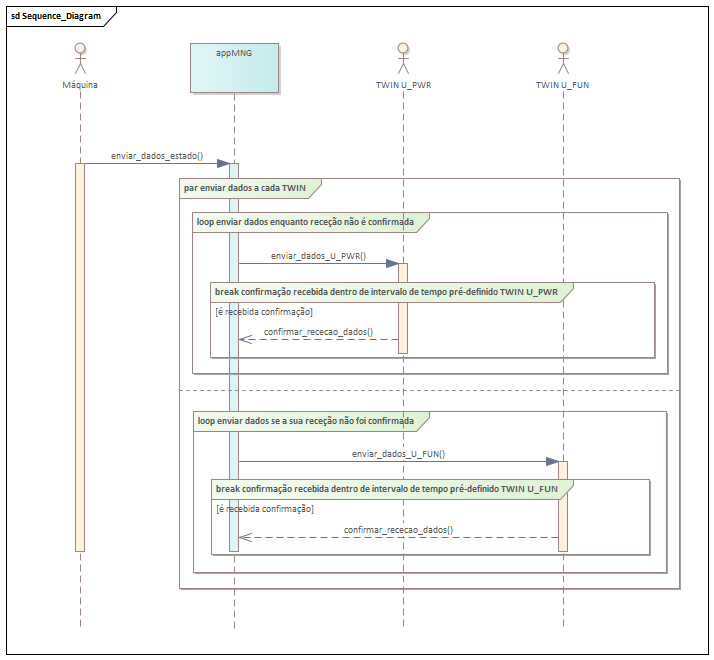
\includegraphics[origin=c, angle=-90]{Sequence_Diagram.png}
    \end{figure}

    \pdfpageattr\expandafter{\the\pdfpageattr/Rotate -90}

    \begin{figure}[H]
        \centering
        \vspace*{-0.3cm}
        \hspace*{-1.80cm}
        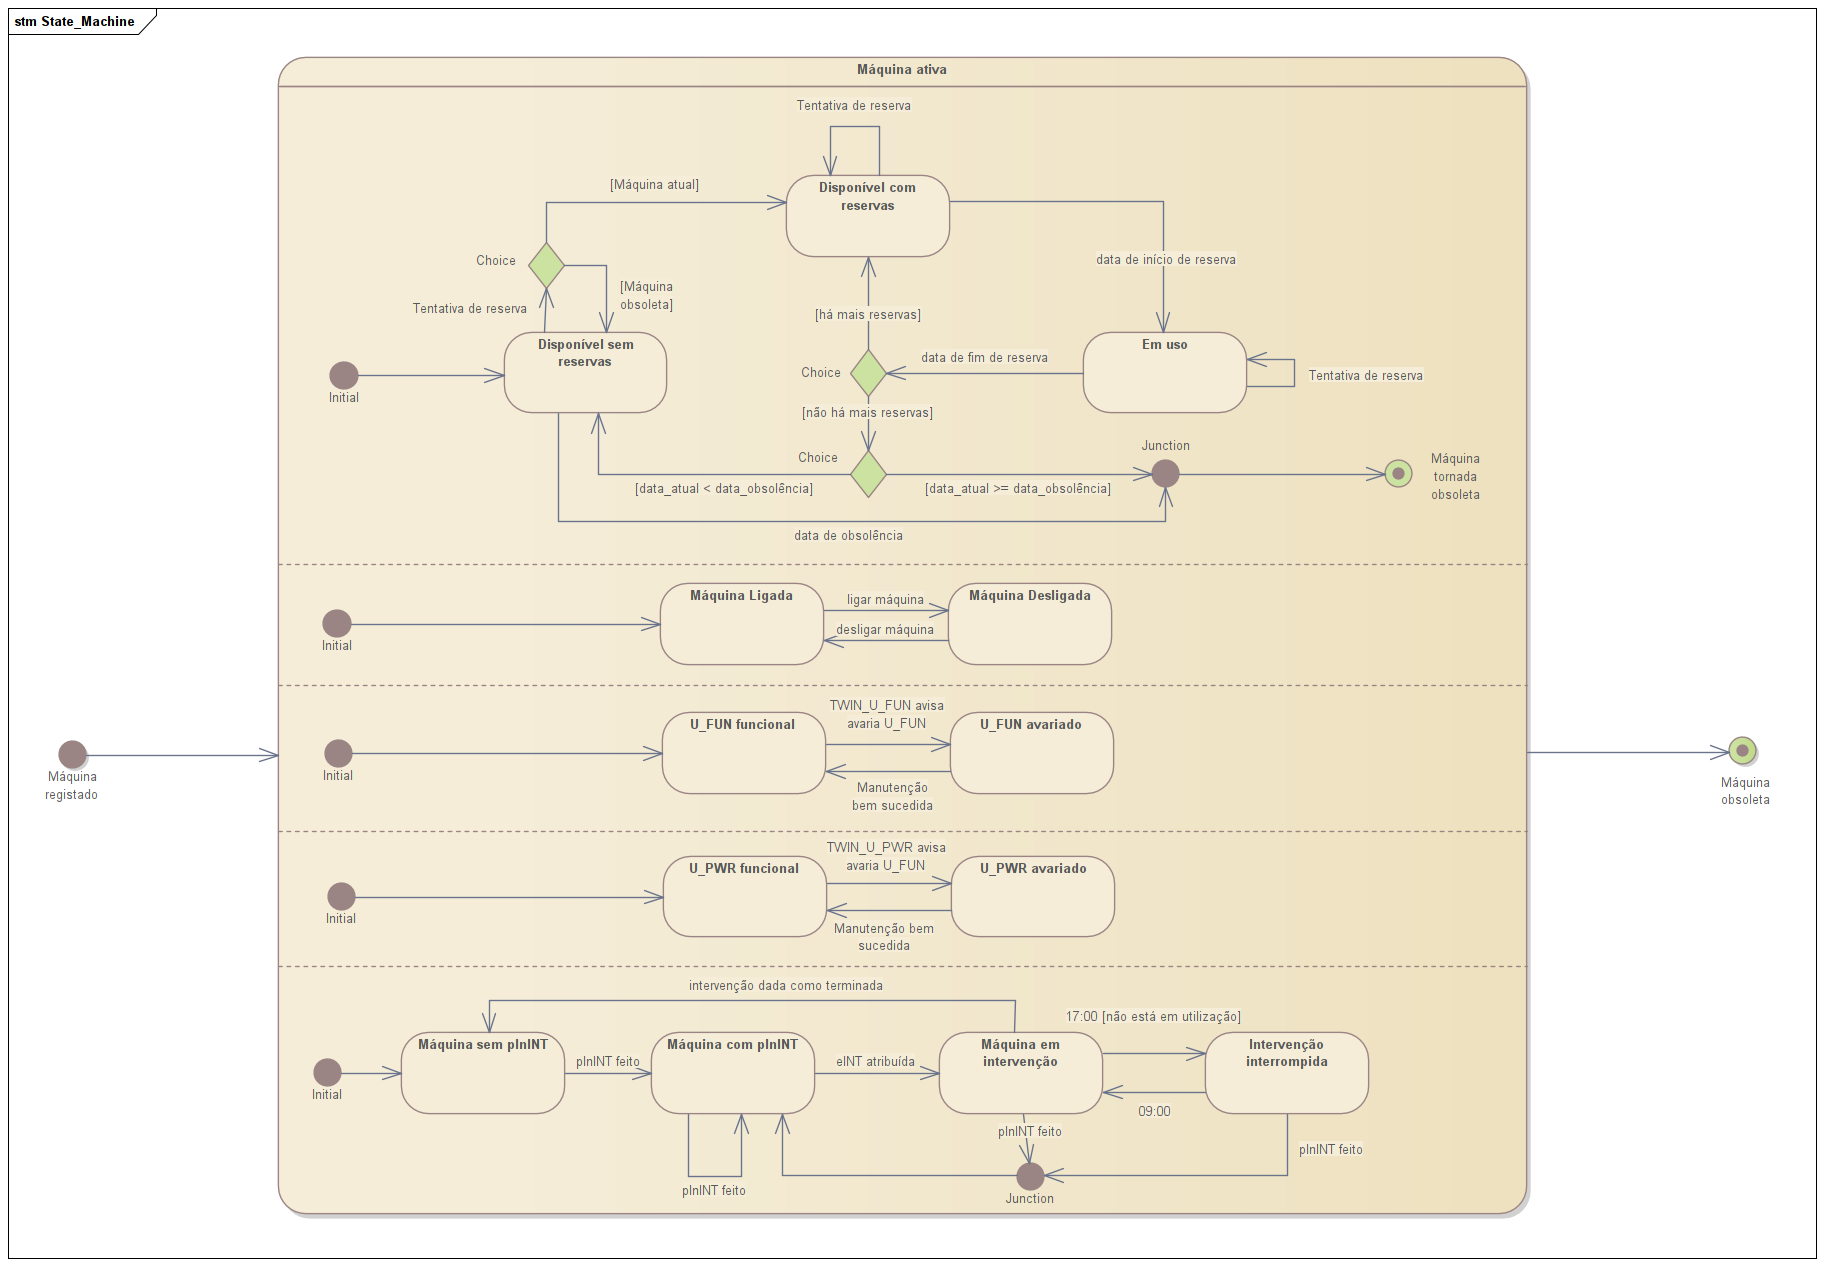
\includegraphics[origin=c, angle=-90, scale = 0.80]{State_Machine.png}
    \end{figure}
%
\end {document}